\documentclass[12pt]{article}

\usepackage{sbc-template}
\usepackage{graphicx,url}
\usepackage{subcaption}
\usepackage[utf8]{inputenc}
\usepackage[brazil]{babel}

     
\sloppy

\title{Análise Comparativa de Desempenho em~\emph{drivers} para MongoDB em Aplicações Node.js}

\author{Leandro Ungari Cayres, Ronaldo Celso Messias Correia }


\address{Faculdade de Ciências e Tecnologia -- Universidade Estadual Paulista (UNESP)\\
  Presidente Prudente -- SP -- Brazil
  \email{\{leandro.ungari,ronaldo.correia\}@unesp.br}
}

\begin{document} 

\maketitle

\begin{abstract}
  This meta-paper describes the style to be used in articles and short papers
  for SBC conferences. For papers in English, you should add just an abstract
  while for the papers in Portuguese, we also ask for an abstract in
  Portuguese (``resumo''). In both cases, abstracts should not have more than
  10 lines and must be in the first page of the paper.
\end{abstract}
     
\begin{resumo} 
  Este meta-artigo descreve o estilo a ser usado na confecção de artigos e
  resumos de artigos para publicação nos anais das conferências organizadas
  pela SBC. É solicitada a escrita de resumo e abstract apenas para os artigos
  escritos em português. Artigos em inglês deverão apresentar apenas abstract.
  Nos dois casos, o autor deve tomar cuidado para que o resumo (e o abstract)
  não ultrapassem 10 linhas cada, sendo que ambos devem estar na primeira
  página do artigo.
\end{resumo}


\section{Introdução}
Nos últimos anos, o crescimento no volume de dados mudou a utilização desses por empresas e organizações; tais dados, inicialmente considerados agentes passivos, relacionados às regras de negócio empresarial; tornaram-se potenciais oportunidades de lucro através da análise de informações, e consequentemente, do conhecimento presente no conjunto de dados.

Essa crescente quantidade de dados, chamado de~\emph{Big Data}, não somente requer maior espaço de armazenamento, mas uma mudança em sua organização com base em cada contexto, considerando características como volume, variedade, velocidade e valores~\cite{ward2013undefined}.
A arquitetura dos tradicionais bancos de dados relacionais, baseada no modelo ACID (\textit{atomicity},~\textit{consistency},~\textit{isolation} e~\textit{durability}), contudo, em ambientes de~\emph{Big Data}, a alta consistência afeta diretamente os aspectos de disponibilidade e  eficiência, que são importantes, devido ao alto volume, variedade e velocidade presente em Big Data~\cite{aparicio:2016}. 

Nesse cenário surgem os banco de dados NoSQL (\emph{Not only SQL}) provendo maior flexibilidade estrutural, suporte a replicação e consistência eventual seguindo o critério BASE (\textit{basic},~\textit{availability},~\textit{soft-state} e~\textit{eventual consistency})~\cite{han2011survey}. 
Nos últimos anos, a popularidade dos banco de dados não-relacionais tem crescido~\cite{cooper2010benchmarking,edlich2015nosql} proporcionando diversas soluções conforme características dos dados cada aplicação.

Diferentemente do modelo relacional, os bancos NoSQL não possuem uma linguagem comum entre eles que permita a realização de operações, como o SQL (\emph{Structured Query Language}), desse modo, cada banco provê uma interface nativa para manipulação dos dados. 
Contudo, uso de chamadas de sistema para execução de comandos dessas interfaces não é reconhecida como uma boa prática, que pode incorrer em diversos problemas. 

De modo a contornar essa situação, para os diferentes ambientes de desenvolvimento e linguagens de programação,~\emph{drivers} tem sido desenvolvidos de modo a viabilizar a execução dos comandos no banco de dados. 
Em muitas situações, a decisão de qual combinação entre banco de dados não-relacional e~\emph{driver} a ser empregada pode ser um problema, devido a variedade de possibilidades, assim como o desconhecimento dos pontos positivos e negativos de cada solução.

Neste artigo, por meio de um estudo comparativo, busca-se avaliar as duas principais soluções de~\emph{drivers} para o MongoDB~\footnote{https://www.mongodb.com/}, respectivamente MongoClient~\footnote{https://mongodb.github.io/node-mongodb-native/} e Mongoose~\footnote{https://mongoosejs.com/}, em ambientes de aplicação Node.js. 
O principal fator considerado para a realização desse análise consiste na definição prévia de esquema para a manipulação dos dados em operações de CRUD (\emph{create}-\emph{read}-\emph{update}-\emph{delete}). Conceitualmente, os banco de dados não-relacionais não requerem esse predefinição, proporcionando flexibilidade, contudo não existe nada que impeça sua utilização, principalmente quanto a respeito do desempenho; possibilitando algum impacto relevante.

A escolha do banco de dados MongoDB ocorreu devido a sua enorme popularidade recente, empregado em diversas aplicações e linhas de pesquisa; o qual consiste na principal opção dentre os bancos de dados que adotam a estratégia de armazenamento orientada a documentos.
A respeito do ambiente Node.js, apesar de uma tecnologia recentes alguns trabalhos apontam a sua viabilidade no desenvolvimento de aplicações~\cite{chaniotis2015node}; além disso, com essa escolha, tanto aplicação quanto banco de dados utilizam JavaScript, permitindo a elaboração de um sistema uniforme, em termos de linguagem de programação.

Na análise conduzida neste trabalho, o desempenho do banco de dados MongoDB atrelado a cada um dos~\emph{drivers} investigados é analisado sobre perspectivas de tempo de execução, tempo de uso de processamento e consumo de memória sob um conjunto de dados genérico, propiciando a identificação de algumas características.

O restante desse trabalho está organizado do seguinte modo: na Seção~\ref{section:nao-relacional} é realiza uma revisão conceitual sobre banco de dados não-relacional, assim como sobre o MongoDB e seus drivers. Na Seção~\ref{section:nodejs} é apresentado o ambiente de execução Node.js assim como detalhes sobre uso de memória que são relevantes no estudo comparativo. A Seção~\ref{section:estudo} é apresentado o estudo comparativo realizado neste trabalho. Seção~\ref{section:resultados} são apresentados os resultados quantitativos obtidos, cuja discussão é elaborada na Seção~\ref{section:discussao}. Em seguida, na Seção~\ref{section:limitacoes} e, por fim, na Seção~\ref{section:consideracoes} as considerações finais desse trabalho.


\section{Banco de Dados Não-Relacional}
\label{section:nao-relacional}

Os bancos de dados NoSQL, , foram desenvolvidos visando armazenar e processar grandes volumes de dados. Em linhas gerais os bancos de dados NoSQL são livres de esquematizações, lidam com dados não estruturados como e-mail, documentos e mídias sociais de maneira eficiente~\cite{mohamed:2014,ramesh:2016}.

O termo NoSQL é comumente utilizado para se referir a uma ampla variedade de armazenamentos de dados nos quais as restrições de transação ACID foram relaxadas para permitir melhor dimensionamento e desempenho horizontal~\cite{rafique:2018}. Os recursos gerais presentes nos bancos de dados NoSQL são sumarizados em: esquemas menos estruturados, suporte a operações de junção, alta escalabilidade, modelagem de dados simples com linguagem de consulta simples~\cite{ramesh:2016}. Os bancos de dados NoSQL foram categorizados em: armazenamento de documentos, famílias de colunas, chave/valor, gráficos e multimodais~\cite{aparicio:2016}.

Este trabalho tem como foco a categoria orientada a documentos, a qual permite a modelagem de dados estreitamente relacionados a programação orientada a objetos. 
Cada documento é considerado como um objeto, da mesma forma cada documento pode ser um JSON ou um XML no banco de dados orientado a documentos. 

O conceito de esquema nos bancos de dados de documentos é dinâmico, uma vez que, cada documento pode conter campos distintos um dos outros, sendo útil na modelagem de dados não estruturados e polimórficos. 
Essa categoria permite consultas robustas, em que qualquer combinação de campos no documento pode ser realizada visando consultar dados~\cite{patil:2017}.
Em termos de estruturação, seus dados são organizados em coleções de documentos, as quais utilizam uma estrutura semelhante a JSON (\emph{JavaScript Object Notation}) ou XML (\emph{Extensible Markup Language}). 

\subsection{MongoDB}

O MongoDB~\cite{membrey2011definitive} é um banco de dados orientado a documentos de código-aberto. Embora são seja considerado um banco de dados relacional, esse apresenta muitas funcionalidades providas por essa categoria, como ordenação, indexação secundária e consultas de intervalo.

A estruturação dos dados não acontece com base em tabelas com suas respectivas colunas e tuplas, mas sim coleções de documentos.
O banco de dados não impõe um esquema, contudo, normalmente todos os documentos em uma coleção são de propósito semelhante ou relacionado~\cite{kanade2014study,lutu2015big}. Há duas abordagens para modelagem de documentos: 

\begin{itemize}
\item Modelo de dados incorporado: os dados relacionados são incorporados em uma única estrutura ou documento. Esses esquemas são geralmente conhecidos como modelos “desnormalizados”.
\item Modelo de dados normalizado: os dados possuem referências de documentos para registrar relacionamentos entre esses, mas a "união" de documentos deve ser feita diretamente no código-fonte da aplicação.
\end{itemize}

O armazenamento dos dados ocorre através da serialização de objetos Javascript, também conhecidos JSON, cuja implementação interna utiliza uma codificação binária chamada BSON~\cite{bson}.

O banco de dados MongoDB disponibiliza diversos~\emph{drivers} para linguagens de programação como Java, C++, C\#, PHP e Python~\cite{lutu2015big}, assim como para aplicações baseadas em Node.js.

Nesse contexto, dentre os~\emph{drivers} existentes, tem-se como destaque o MongoClient~\footnote{https://mongodb.github.io/node-mongodb-native/index.html}, consiste na solução oficial e nativa provida organização, provendo um conjunto de funcionalidades que permite a manipulação dos dados e uso de recursos avançados do sistema. 
Essa solução é caracterizada pela modelagem documentos-objeto (\emph{ODM -- Object-Document Modeler}) de modo implícito ao banco de dados.

Assim como o anterior, o Mongoose consiste também em um driver para MongoDB, porém esse provê a modelagem de dados utilizando um mecanismo semelhante ao mapeamento de dados em tabelas (\emph{ORM -- Object Relational Mapping}) utilizado em banco de dados relacionais~\cite{mardan2014boosting}, executando diversas tarefas de verificação e validação dos dados, como nulidade ou tipagem, previamente definidos por meio da elaboração de um esquema.

\section{Node.js}
\label{section:nodejs}

Node.js é uma plataforma construída sob o ambiente de execução para JavaScript do navegador Google Chrome, para criação facilitada de aplicações de internet rápidas e escaláveis~\cite{nodejs}. 
Esse ambiente se baseia em mecanismo orientado a eventos de entrada e saída não-bloqueante, o que viabiliza a interação do usuário enquanto demais tarefas executam em segundo-plano, resultando em aplicações leves e eficientes.

Atualmente, pode ser observado um crescente número de projetos utilizando essa tecnologia, o que é comprovado pela popularidade da plataforma desde as suas versões iniciais, atrelada a crescente utilização da linguagem Javascript~\footnote{https://github.com/search?l=JavaScript\&o=desc\&q=stars\%3A\%3E1\&s=stars\&type=Repositories}.

\subsection{Organização de Memória em Aplicações Node.js}

Toda aplicação Node.js em execução, assim como qualquer processo em geral, requer que uma região da memória seja reservada. 
A Figura~\ref{figure:memoria} apresenta a organização da memória em processos Node.js.

\begin{figure}[h]
    \centering
    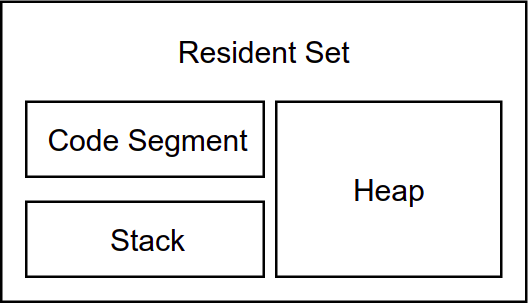
\includegraphics[width=0.4\textwidth]{images/set}
    \caption{Organização de memória de um processo Node.js -- adaptado de~\cite{nodememory}.}
    \label{figure:memoria}
\end{figure}

A primeira região, que engloba as demais, é chamada~\emph{Resident Set}, essa corresponde a toda memória utilizada no processo. 
Em seguida tem-se a região~\emph{Code Segment}, a qual armazenada todas as instruções definidas para o programa.
A proxima região~\emph{Stack} armazena todas as variáveis e estruturas de dados utilizadas durante o tempo de vida dessas.
Por fim, tem-se a região~\emph{Heap}, a qual armazena dados específicos como objetos, strings e closures; em geral, cada processo aloca esse região com um tamanho predefinido, contudo essa pode ser utilizada apenas parcialmente ou em sua totalidade~\cite{nodememory}. 

\section{Estudo Comparativo}
\label{section:estudo}

Nesta seção é apresentado o estudo realizado comparando os~\emph{drivers}MongoClient e Mongoose, conforme apresentado na Figura~\ref{figure:diagrama-banco}. 

\begin{figure}[ht]
    \centering
    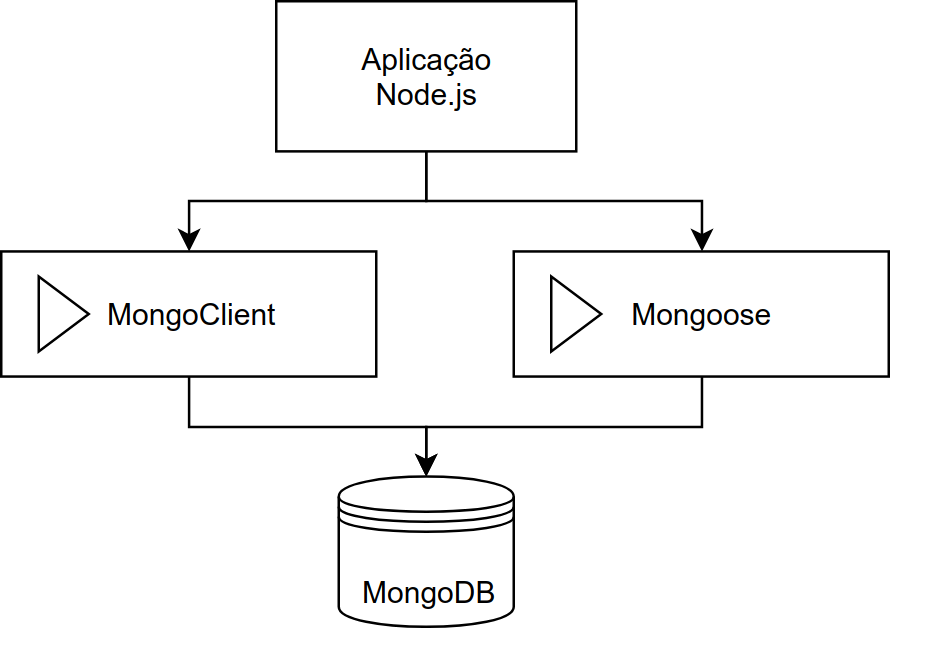
\includegraphics[width=0.6\textwidth]{images/diagram-banco}
    \caption{Estudo de caso para comparação dos drivers.}
    \label{figure:diagrama-banco}
\end{figure}

A ideia principal consiste em analisar ambos sob o desempenho médio, em termos de algumas métricas, na execução das operações que compõem o CRUD, de modo avaliar o real impacto sob um mesmo cenário em termos de banco de dados e aplicação utilizada.

Como principal ponto de diferença entre os~\emph{drivers} consiste na modelagem dos dados, neste estudo, foram conduzidas análises visando identificar se o tamanho médio de cada registro pode influenciar e qual a proporção desse impacto.

As métricas escolhidas para análises de cada um dos cenários conduzidos foram as seguintes:
\begin{itemize}
\item Tempo de Execução Médio: consiste tempo médio total de execução de cada operação específica.
\item Tempo de Processamento Médio: consiste no tempo médio de uso do processador durante a execução da operação específica.
\item Variação Média de Uso de Memória: consiste na variação média de uso de memória RAM durante a execução da operação específica, sendo expressa em kilobytes (KB).
\end{itemize}

Por fim, os resultados obtidos em cada um dos cenários analisados são apresentados na Seção~\ref{section:resultados} e discutidos na Seção~\ref{section:discussao}, com base nas seguintes questões de pesquisa:

\textbf{Q1} --~\emph{O tamanho médio dos registros impacta de modo relevantes quanto ao uso de memória nas operações de CRUD?}

\textbf{Q2} -- O tamanho médio dos registros pode influenciar no uso de CPU nas operações de CRUD? 

\textbf{Q3} -- O tamanho médio dos registros impacta no tempo de execução de cada uma das operações de CRUD?


\subsection{Dataset}

O presente estudo utilizou um conjunto de dados com cerca 18 mil instâncias de dados, proveniente do seguinte dataset~\footnote{https://www.kaggle.com/karangadiya/fifa19}.
Originalmente, todos os registros presentes são compostos por 89 atributos, predominante textuais, obtendo um tamanho médio de 1,37KB.
A partir do conjunto original, foi construído um conjunto reduzido em número de atributos (6 atributos), com o mesmo total de instância, porém com tamanho médio de 0,13KB.


\subsection{Ambiente de Execução}

O ambiente de execução para os testes de desempenho consistiu em um computador pessoal com sistema operacional Ubuntu 18.04.2, processador Intel i3 3217U e memória RAM de 4GB. 

Durante a execução dos testes, o ambiente de execução da aplicação Node.js foi definido o uso do~\emph{heap} de memória com limite máximo de 3GB, o que restringiu no limite superior do número de operações executadas em cada cenário de teste.

Em cada cenário de execução, foram extraídos dados relativos ao tempo de execução, tempo de uso de CPU e uso de memória RAM.
Foram analisados cenários com diferentes quantidades de operações CRUD realizadas, as quais variaram de 1000, 10000, 100000 e 200000; cada qual foi repetido 10 vezes. 

A obtenção das métricas de desempenho de cada um dos cenários, para tempo de execução, tempo de uso de CPU e memória RAM, foi realizada através da biblioteca JSMeter~\footnote{https://github.com/wahengchang/js-meter}. 

\subsection{Resultados}
\label{section:resultados}

Todos os resultados a seguir são apresentados sob a perspectiva que cada uma das operações (\emph{create}-\emph{read}-\emph{update}-\emph{delete}) respectivamente, em que 100\% dos registros são atingidos em cada operação. 
Cada resultado apresenta o tempo de execução, em uma operação específica, da combinação de um~\emph{driver} com o conjunto de dados pequeno (referente ao dataset original com todos atributos) ou grande (referente ao dataset com número reduzido de atributos).

\begin{figure}[ht]
\centering
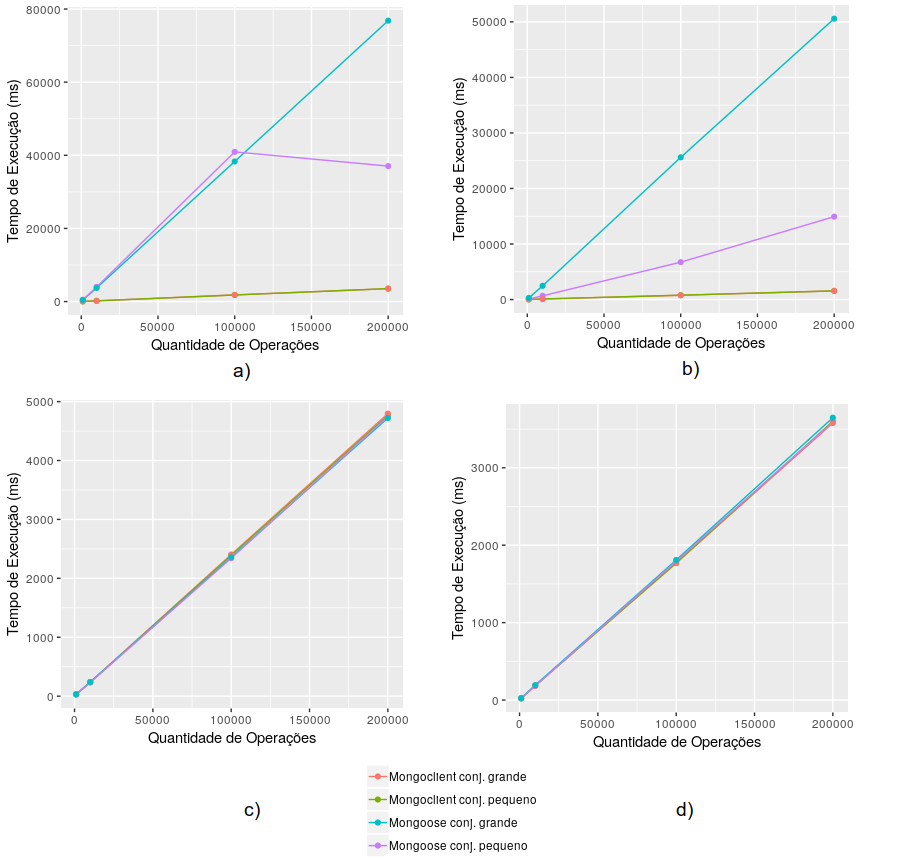
\includegraphics[width=\textwidth]{images/time}
\caption{Comparativo de operações em relação ao tempo de execução.}
\label{fig:time}
\end{figure}

A primeira análise, na Figura~\ref{fig:time}, apresenta os resultados relativos ao tempo de execução. 
A Figura 3a apresenta, para operação de inserção, o tempo de execução do~\emph{driver} Mongoose maior, para os dois conjuntos, de modo relevante, enquanto para o MongoClient, aparenta não haver diferenças significativas entre os conjuntos. 
Como exceção, pode-se observar a execução do conjunto pequeno para o Mongoose, em que o tempo para 200 000 operações não mantém a proporcionalidade das demais execuções. Um possível fator que justifique esse comportamento consiste na ocorrência de divisão de conjuntos na operação de inserção quando a quantidade excede 100 000 itens, contudo, isso não ocorre para o conjunto de registros grandes.

A Figura 3b também apresenta, para operação de busca, o tempo de execução inferior para ambos os conjuntos do MongoClient, em que ambos atuam de modo estritamente similar. 
Quanto ao Mongoose, as execuções para conjunto reduzido e grande apresentam comportamente crescente e proporcional em detrimento a diferença de tamanho dos registros. 

As Figuras 3c e 3d, para as operações de atualização e deleção de registros, ambos os~\emph{drivers} para os conjuntos obtiveram tempos de execução estritamente similares e proporcionando a quantidade de operações, não apresentando diferenças significativas, nem mesmo quanto ao tamanho médio dos registros.

\begin{figure}[ht]
    \centering
    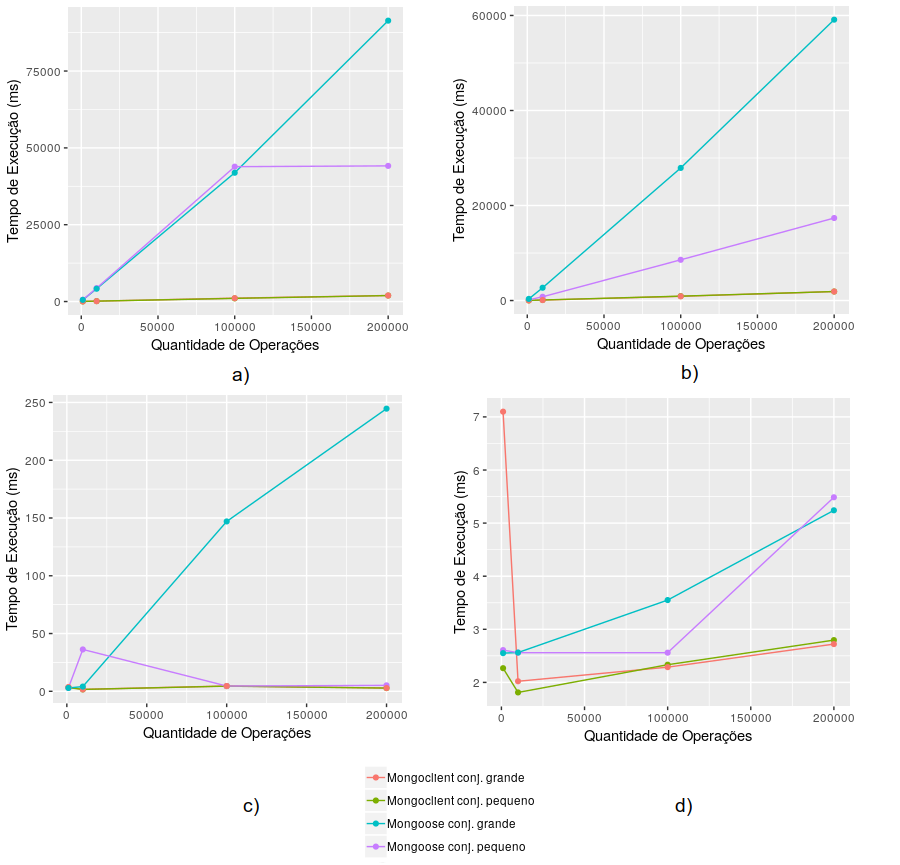
\includegraphics[width=\textwidth]{images/cpuusage}
    \caption{Comparativo de operações em relação ao tempo de uso do processador.}
    \label{fig:cpuusage}
\end{figure}

A próxima análise, na Figura~\ref{fig:cpuusage}, é referente aos resultados relacionados ao tempo de uso de processamento em cada operação.
As Figuras 4a e 4b, assim como análise anterior, para as operações de inserção e busca, apresenta o MongoClient com tempo de execução médio significativamente inferior, em ambos os conjuntos, em detrimento do alto tempo apresentado pelo Mongoose.

A Figura 4c, representa a operação de atualização, em que se pode-se observar somente o~\emph{driver} Mongoose com conjunto de registros maiores apresentou maior tempo de uso de processamento, em detrimento dos demais, que foram semelhantes e com tempo menor relevantemente, mesmo com oscilações. 
É importante salientar que o tempo de processamento de todas as execuções foram inferiores a 250ms.
A Figura 4d, representa a operação de deleção, cada execução apresentou comportamento relativamente instável, tendo as execuções com~\emph{driver} com tempo um pouco maior, contudo não há diferença significativa, porque todas as execuções obtiveram tempo de processamento inferior a 10ms.

\begin{figure}[ht]
    \centering
    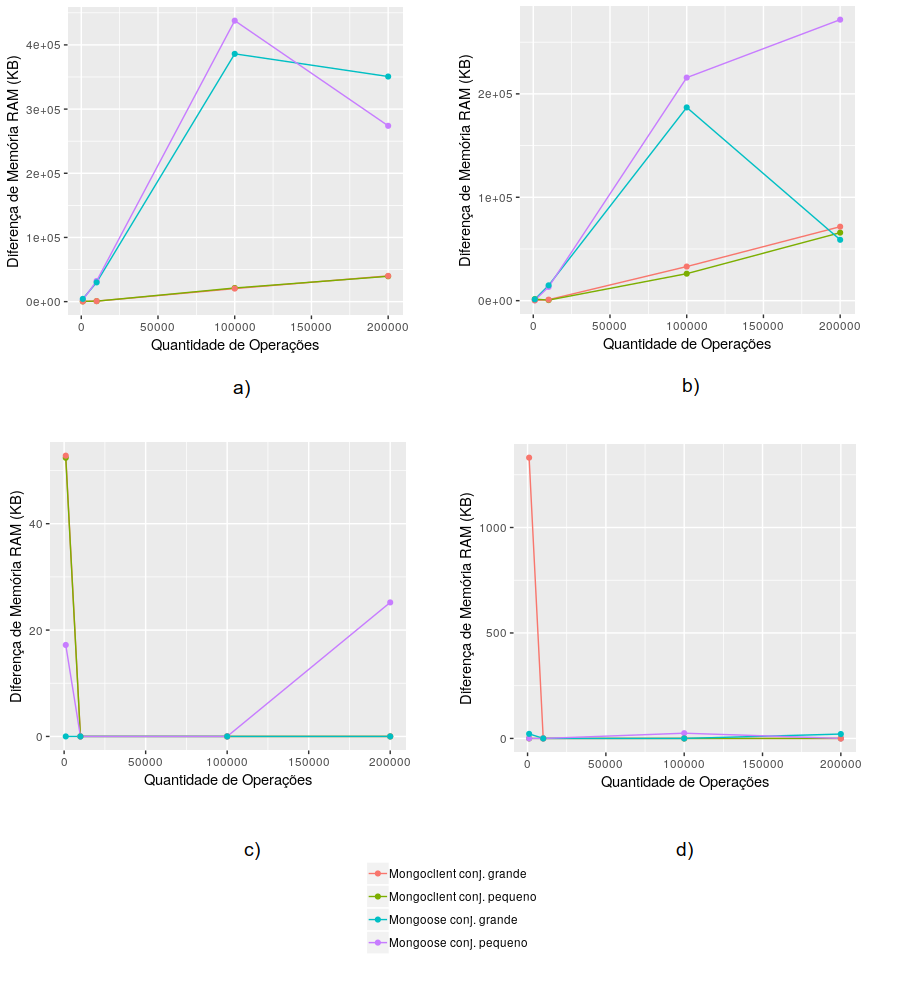
\includegraphics[width=\textwidth]{images/memory}
    \caption{Comparativo de operações em relação ao uso de memória.}
    \label{fig:memory}
\end{figure}

A última análise, apresentada na Figura~\ref{fig:memory}, refere-se a variação média do uso de memória RAM em cada operação. 



\section{Discussão dos Resultados}
\label{section:discussao}

\subsection{Discussão da Q1}

\subsection{Discussão da Q2}

\subsection{Discussão da Q3}


\section{Ameaças à Validação}
\label{section:limitacoes}



\section{Trabalhos Relacionados} 
\label{section:relacionados}

\cite{kanade2014study} did a study for NoSQL databases with both normalized and denormalized forms using a similar dataset, and have found that the embedded MongoDB
data model provides a much better efficiency as compared to a normalized model. 


\section{Considerações Finais}
\label{section:consideracoes}

\section{Referências Bibliográficas}

\bibliographystyle{sbc}
\bibliography{sbc-template}

\end{document}
